

\subsection{Einfeldt Strong Rarefaction Test}

This test measures the solver's vulnerability to very strong rarefactions that can, in some cases, 
produce negative mass densities or pressures. The input parameters can be tweaked slowly to determine 
exactly how strong the rarefaction can become before producing values that are NAN. 

\subsubsection{Analysis}

\begin{figure*}
\begin{center}
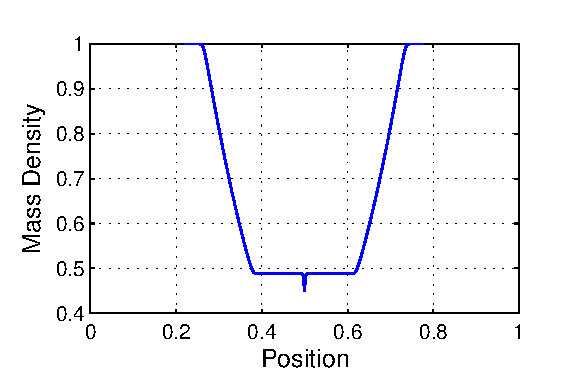
\includegraphics{Einfeldt.eps}
\caption{Einfeldt test at t = 0.1}
\end{center}
\end{figure*}
\subsubsection{Initial Conditions}

Boundary conditions are constant around the X axis and periodic everywhere else.

Einfeldt's Strong Rarefaction test consists of a 1-dimensional grid divided exactly in half. The 
properties of each half are defined separately, using four physical parameters. When run, the test 
produces two strong rarefaction waves moving away from the midpoint of the grid.

The physical input parameters to the Einfeldt Strong Rarefaction test are:
\begin{itemize}
\item \tt{rho} - Defines the mass density of the region
\item \tt{m} - Defines the X-momentum of the region (parallel to the grid)
\item \tt{n} - Defines the Y-momentum of the region (perpendicular to the grid)
\item \tt{e} - Defines the energy density of the region
\end{itemize}

The four parameters are saved separately as rhol and rhor, ml and mr, and so on.
